%\chapter{Empirical Work}


\chapter{Interviews with Working Professionals}

\section{Problem Identification \& Motivation}
\section{Definition of Solution Objectives}
\section{Summary}



\chapter{GitOps Promotions Operator Prototype}

This chapter describes the developed prototype,
called the GitOps Promotions Operator.

\section{Design \& Development}

The Design of the GitOps Promotions Operator
is based on the underlying conditions of the Kubebuilder framework,
discussed in section \ref{theoretical-background:kubernetes} of this thesis.
The main conditions the framework comes with, are the
custom resource definition + controller pattern.

\begin{figure}[h]
	\centering
	
\includegraphics[width=1.00\linewidth]{assets/crd-and-controller.png}
	\caption{Custom Resource Definition and Controller.
		%		(\citeauthor{ref}, \citeyear{ref}).
	}
	\label{fig:crd-and-controller}	
\end{figure}

\subsection*{Abstract Models}
	
The first step of the initial design phase is the creation abstract models.
In order to be able to represent environments and promotions,
the requirements is at least two abstractions models for each 
the environment and promotion.

The Environment represents a GitOps environment,
which is a Git repository + path.
The Git repository can be a clone URL to the repository,
and the path is the relative filesystem path, which points to the 
environment, inside the repository.

\begin{figure}[h]
	\centering
	
\includegraphics[width=1.00\linewidth]{assets/gitops-env-repo-and-path.png}
	\caption{GitOps Environment.
		%		(\citeauthor{ref}, \citeyear{ref}).
	}
	\label{fig:gitops-env-repo-and-path}	
\end{figure}

The abstract model for a GitOps environment needs at least the following properties:

\begin{itemize}
	\item URL of the source Git repository
	\item path pointing to the environment inside the repository
\end{itemize}

The URL has the format of a HTTP(S) or SSH URL,
which links to the Git repository,
e.g.:

\begin{itemize}
	\item \verb*|http://localhost:8080/org/repo|
	\item \verb*|https://gitprovider.com/org/repo|
	\item \verb*|ssh://git@gitprovider.com:org/repo|
\end{itemize}

The path has the format of a typical unix style filesystem path.
It starts relative from the root of the given Git repository,
and points to the directory, which represents the GitOps environment.
Examples for a path are the following:

\begin{itemize}
	\item \verb*|path/to/env|
	\item \verb*|/path/to/env|
	\item \verb*|./path/to/env|
	\item \verb*|./path/to/env/|
\end{itemize}

Note, that these example paths all represent the same directory.

The abstract model for a GitOps promotion needs at least the following properties:

\begin{itemize}
	\item source environment
	\item target environment
	\item promotion subjects
	\item promotion strategy
\end{itemize}

The source environment defines the environment resource,
where a promotion subject is promoted from.
The target environment defines the environment resource,
where a promotion should promote to.

A promotion subject can be potentially many different things.
In the case of this prototype development,
a promotion subject is a file or directory,
which is copied from the source to the target environment.
Examples of such files or directories are the following:

\begin{itemize}
	\item kustomization.yaml
	\item ./component/cert-manager/kustomization.yaml
	\item ./helm-values-prod.yaml
\end{itemize}

A promotion subject could also be fetched from another source,
like an artifact registry,
and updated/promoted in the target environment,
e.g. a version tag.

The promotion strategy can be a git pull request.
A pull request will be created with the changes a promotion would do, 
which can be reviewed by a human,
and approved and accepted/merged.
Only after a pull request is merged,
the promotion will take effect, and the subjects are promoted to the target environment.

Alternatively to a pull request, the changes could be directly
commited and pushed to the target environment,
without human interaction. This strategy should require different means
of automated or otherwise external checks, in order to ensure a safe promotion.

The abstract models which are designed,
need to be implemented.
Since the Kubebuilder framework -
this prototype is developed with -
already offers declarative APIs
in the form of custom resource definitions,
the implementation is focused on the content itself.
The technological boundaries are given by the framework.





\subsection*{Mockups of Custom Resources}

%to write mockups
%of custom resources in YAML format,
%since this is what the end user will interface with when the application is finished.
%First and foremost the handling and user experience has to be seamless and make sense
%for the user; also it shouldn't take any extra miles for the user to take,
%just to get started.
%The YAML representation of the custom resource should be similar to other ones
%from the Kubernetes core types.

When the abstract models have been specified,
they can be actually implemented with the framework
as Kubernetes custom resource definitions.

Users will mainly be dealing with the custom resources in a Yaml format.
Yaml keys should be intuitive and make sense to the user.
It also helps if they follow the core Kubernetes definitions,
e.g. regarding naming conventions.
An example for a naming convention is the "Ref" suffix for yaml keys.
This suffix is appended to keys which represent a reference to another Kubernetes
object.
For example, "secretRef" says that this field refers to a Kubernetes secret resource.

A possible mockup for a GitOps environment -
that is a first prototype implementation of the abstract model into a custom resource -
could look like the following.

\verbatiminput{assets/files/environment-mockup.yaml}

In this mockup the git reference branch main is also specified \\
in the \verb*|.spec.source.ref.branch| field.

A possible mockup for a GitOps promotion 
could look like the following.

\verbatiminput{assets/files/promotion-mockup.yaml}

In the promotion mockup definition,
there are four main fields within the \verb*|.spec|.
These represent the minimum properties of our abstract definition.
It is to note, that
the \verb*|.spec.copy| field represents the promotion subjects.
It is a list of items, where each item contains
a \verb*|name|, \verb*|source| and \verb*|target|.
The \verb*|name| defines a custom name.
The \verb*|source| and \verb*|target| fields together define a
file copy operation,
where the \verb*|source| is the relative path from the source environment,
and the \verb*|target| is a relative path from the target environment.

\subsection*{Alternative Mockups}

The following alternative mockups,
for the custom resource definitions,
i.e. the design of the declarative API,
are suggested.

\subsubsection*{Promotion Subjects decoupled from Promotion resource}

Alternatively, the promotion subjects could also be specified
in the environment resource.
Then the environment could like the following:

\verbatiminput{assets/files/environment-mockup-alt-1.yaml}

In the promotion definition,
it would then suffice to specify
a list of promotion subjects.

\verbatiminput{assets/files/promotion-mockup-alt-1.yaml}












\section{Proof-of-Concept Demonstration}
\section{Evaluation Of Proof-of-Concept Use Cases}
\section{Summary}







%\chapter{Interviews with Working Professionals}
%
%\section{Categorisation of Findings}
%\section{Common Problem Definitions}
%\section{...?}
%
%
%\chapter{Definition of Solution Objectives}
%
%\section{People \& Communication Perspective}
%\section{Technical Perspective}
%\section{...?}
%
%
%\chapter{Prototype Design and Development}
%
%\section{Architecture}
%\section{Functionality}
%\section{...?}
%
%\chapter{Proof-of-Concept Demonstration}
%
%\section{Setup and Use with Kustomize}
%\section{Setup and Use with Helm}
%\section{Multiple Environments in same Stage}
%\section{Scalability}
%\section{...?}















%
%\section{Instruction included in the original FHBgld word processor template}
%Die Durchführung der empirischen Untersuchung ist nachvollziehbar zu dokumentieren sowie auch die dabei aufgetretenen Probleme und deren Behandlung. Der Umfang ergibt sich aus der Art der Bearbeitung.  
%
%Tabelle 1 zeigt ein Bespiel für eine Tabelle. 
%
%\begin{figure}[ht]
%	\centering
%	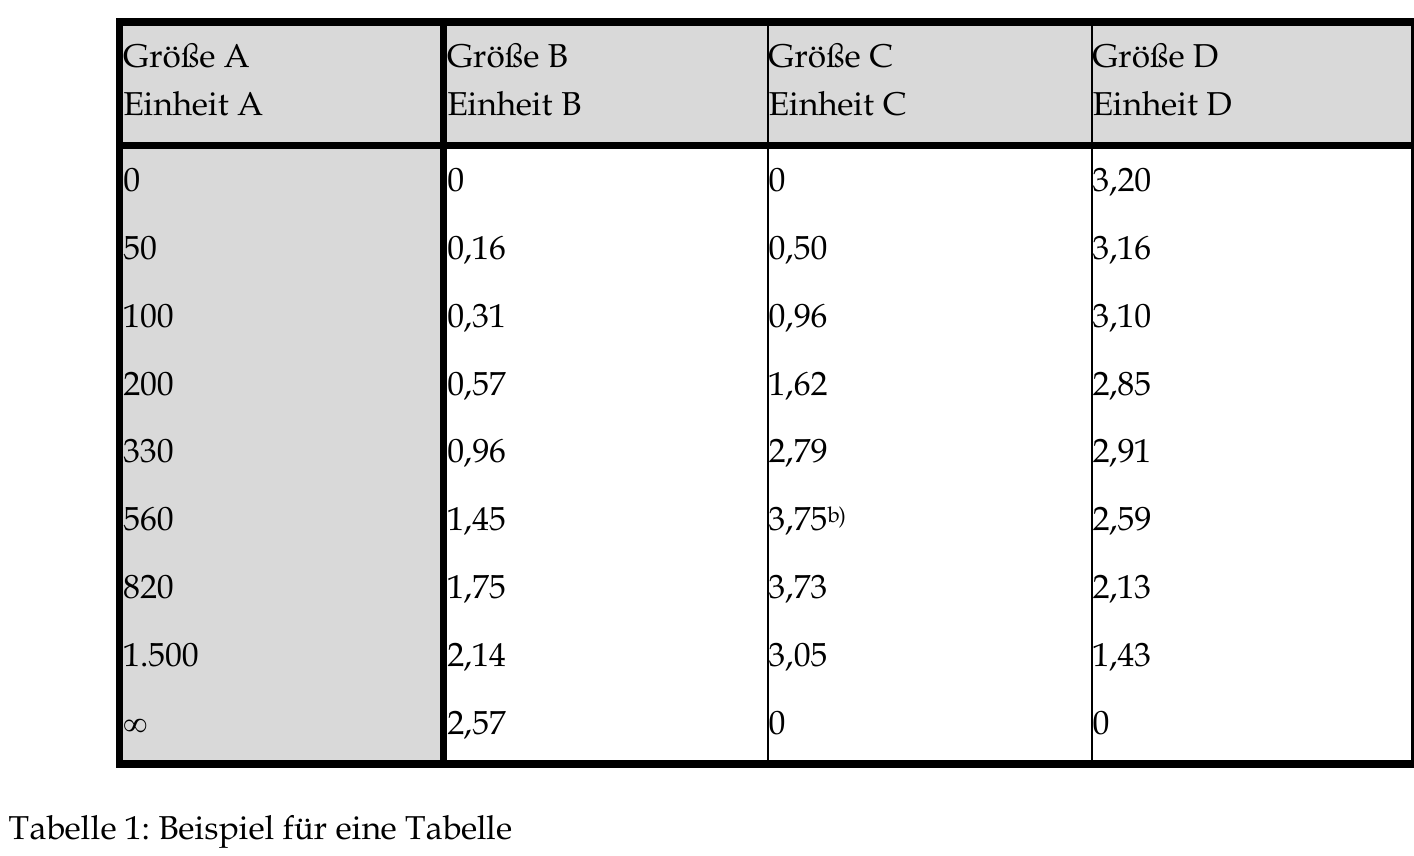
\includegraphics[width=0.7\linewidth]{figures/Word_Table}
%	\caption{Screenshot example from FHBgld word processor template}
%	\label{fig:wordtable}
%\end{figure}
%Abbildung 1 zeigt ein Beispiel für eine Abbildung oder Grafik.
%\begin{figure}
%	\centering
%	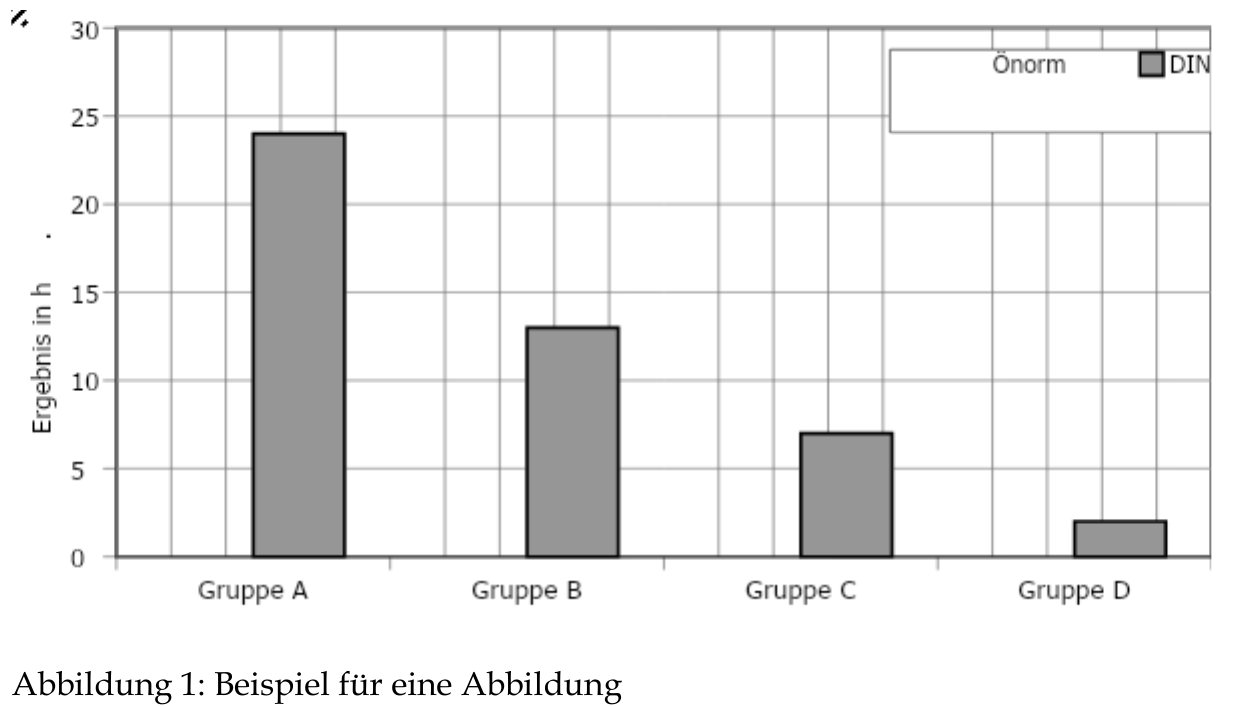
\includegraphics[width=0.7\linewidth]{figures/Word_Diagram}
%	\caption{Screenshot example from FHBgld word processor template}
%	\label{fig:worddiagram}
%\end{figure}
%\linebreak
%Mathematisch werden die Zusammenhänge wie im Figure \ref{fig:wordformel} beschrieben.
%\begin{figure}
%	\centering
%	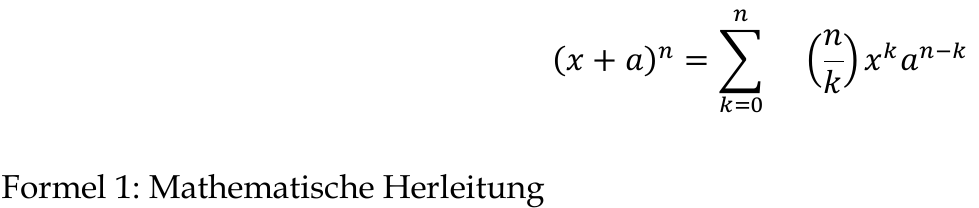
\includegraphics[width=0.7\linewidth]{figures/Word_Formel}
%	\caption{Screenshot example from FHBgld word processor template}
%	\label{fig:wordformel}
%\end{figure}
%
%\section{Tables and Images with \LaTeX}
%One of the great advantages of \LaTeX{} is that all it needs to know is
%the structure of a document, and then it will take care of the layout
%and presentation itself.  So, here we shall begin looking at how exactly
%you tell \LaTeX{} what it needs to know about your document.
%
%\subsection{Tables}
%In this sub-section, a simple table is inserted. To add reference to the table, see (cf. Table~\hyperref[tab:tableexample0]{\ref{tab:tableexample0}}):
%
%%A simple table.  The center environment is first set up, otherwise the
%%table is left aligned.  The tabular environment is what tells Latex
%%that the data within is data for the table.
%% https://en.wikibooks.org/wiki/LaTeX/Tables
%\begin{table}[htb]
%	\begin{tabular}{|b{7cm}|c|}
%		%The tabular environment is what tells Latex that the data within is
%		%data for the table.  The arguments say that there will be two
%		%columns, both left justified (indicated by the 'l', you could also
%		%have 'c' or 'r'.  The bars '|' indicate vertical lines throughout
%		%the table.
%		
%		\hline  % Print horizontal line
%		\fontsize{11pt}{12pt}\selectfont Command & Level \\ \hline  % Columns are delimited by '&'.  And
%		%rows are delimited by '\\'
%		\fontsize{10pt}{14pt}\selectfont Some sections to provide some examples: & \\
%		\texttt{\textbackslash part\{\emph{part}\}} & -1 \\
%		\texttt{\textbackslash chapter\{\emph{chapter}\}} & 0 \\
%		\texttt{\textbackslash section\{\emph{section}\}} & 1 \\
%		\texttt{\textbackslash subsection\{\emph{subsection}\}} & 2 \\
%		\texttt{\textbackslash subsubsection\{\emph{subsubsection}\}} & 3 \\
%		\texttt{\textbackslash paragraph\{\emph{paragraph}\}} & 4 \\
%		\texttt{\textbackslash subparagraph\{\emph{subparagraph}\}} & 5 \\
%		\hline
%		
%	\end{tabular}
%	\caption{some description of the table}
%	\label{tab:tableexample0}
%\end{table}
%
%\subsubsection{More tabular examples}
%
%First, a plain simple example for a FHBgld table, see table~\hyperref[tab:tab:tableexample1]{\ref{tab:tableexample1}}.
%
%\begin{table}[h]
%	\centering
%	\begin{tabular}{|b{1cm}|b{2cm}|b{3cm}|b{4cm}|}
%		\hline
%		\multicolumn{4}{|l|}{\fontsize{11pt}{12pt}\selectfont\noindent First line in 11pt fontsize } \\ \hline
%		1cm & 2cm & 3cm & 4cm \\ \hline
%		from & here on & the table & font size \\ \hline
%		will & be as & defined & in class, that is 10pt\footnote{yes, really!} \\ \hline
%		will & be as & defined & in class, that is 10pt\footnote{yes, really!} \\ \hline
%		will & be as & defined & in class, that is 10pt\footnote{yes, really!} \\ \hline
%		will & be as & defined & in class, that is 10pt\footnote{yes, really!} \\ \hline
%		will & be as & defined & in class, that is 10pt\footnote{yes, really!} \\ \hline
%	\end{tabular}
%	\caption{some description of the table}
%\label{tab:tableexample1}
%\end{table}
%
%Next, a table with nine columns, see table~\hyperref[tab:tableexample2]{\ref{tab:tableexample2}}.
%
%\begin{table}[h]
%	\centering
%	\begin{tabular}{|*{9}{l|}}
%		\hline
%		{\fontsize{11pt}{12pt}\selectfont This} & {\fontsize{11pt}{12pt}\selectfont table} & {\fontsize{11pt}{12pt}\selectfont has} & {\fontsize{11pt}{12pt}\selectfont way} & {\fontsize{11pt}{12pt}\selectfont too } & {\fontsize{11pt}{12pt}\selectfont many} & {\fontsize{11pt}{12pt}\selectfont columns}, & {\fontsize{11pt}{12pt}\selectfont does'nt} & {\fontsize{11pt}{12pt}\selectfont it?} \\ \hline
%		One & Two & Three & Four & Five & Six & Seven & Eight & Nine! \\ \hline
%		At & least & the & first & column & has & 11pt & font & size. \\ \hline
%	\end{tabular}
%	\caption{some description of the table}
%	\label{tab:tableexample2}
%\end{table}
%
%\subsection{Images}
%% Here is how to insert an image as a figure. There is a lot more you can do
%% when inserting images, check out: https://en.wikibooks.org/wiki/LaTeX/Importing_Graphics
%
%\begin{figure}[h]
%	\centering
%	
\includegraphics[width=0.3\textwidth]{figures/logo_nontransparent.jpg}
%	\caption{Image Example}
%	\label{fig:image_example}
%\end{figure}
%
%When an image is inserted, you can refer to it like this (cf. Figure~\hyperref[fig:image_example]{\ref{fig:image_example}}).
%
%\subsubsection{A Subsubsection}
%As one last example, this is how you can insert a sub-sub-section! Have fun
%writing your thesis with \LaTeX{}!
%
%\lipsum[2-3]
%\raggedbottom
%
%\pagebreak
